\chapter{識別器}\label{abst}

\section{サポートベクタマシーンの概要}
サポートベクタマシーン(Support Vector Machine : SVM)は教師あり学習を用いるパターン認識モデルの一つ[3]である.
主にパターン認識や回帰分析に適用されることが多い.SVMは,基本的には線形しきい素子を用いて,
2クラスのパターン識別器を構成する手法である.そのため,文字認識などの多クラスの識別器を構成する場合には,
複数のSVMを組み合わせる必要がある.また,あらかじめ与えられたデータを分類するだけでなく,
未学習データに対して高い識別性能を得ることができるという特徴がある.一般的にはクラス分類において,
データの次元数が多いとデータの分類性能は悪くなるが,SVMでは,データの次元数が多くても性能低下が少ない.
カーネル法を用いることにより,非線形の識別関数を構成できるように拡張することも可能である.

このように,SVMは現在知られている多くの手法の中でも2クラスのパターン認識においては,
最も認識性能の優れた学習方法の一つであり,様々な応用問題を解決できる可能性を持っている.

\section{線形クラス分類}
SVMは,ニューラルネットワークに使用されているパーセプトロンと基本構造が同じ分類器である.
そのパーセプトロンの中でも最も単純な線形しきい素子を用いて,2クラスのパターン識別器を構成する.
線形しきい素子は,図\ref{fig:senkeisoshi}に示すようなニューロンを単純化したモデルであり,入力特徴ベクトル に対して,
式(4.1)の識別関数(線形識別関数)により,2値の出力値を計算する.

\newpage

\begin{figure}[htbp]
  \begin{center}
    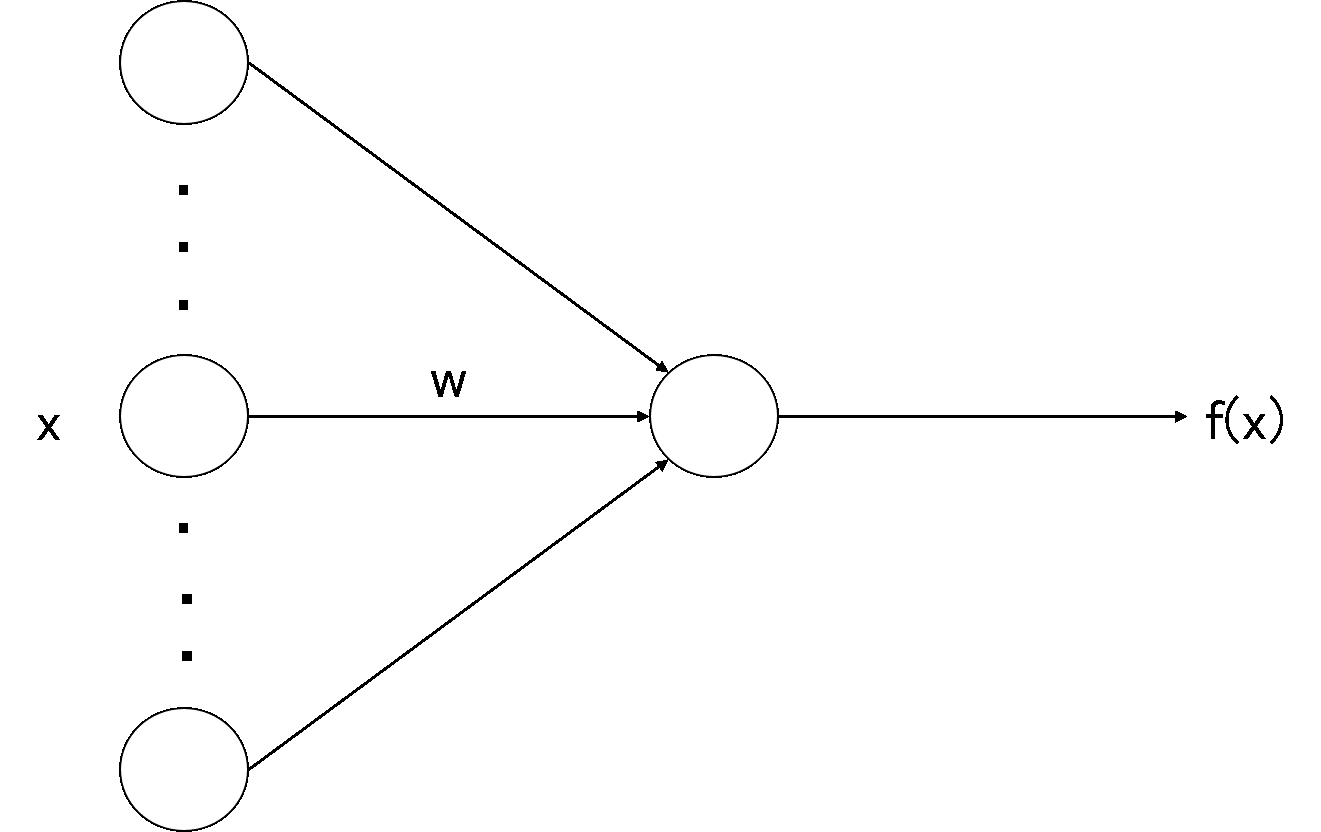
\includegraphics[clip,width=7.0cm]{./images/senkeisoshi.png}
    \caption{線形しきい素子}
    \label{fig:senkeisoshi}
  \end{center}
\end{figure}

\begin{equation}
     f(x) = \sin \{ (w \cdot x) + b \}
\end{equation}

ここで,$w$はシナプス荷重に対応するパラメータであり, はしきい値である. と によって関数は制御されるため,
学習によって求めるべきパラメータである.また,関数sin(u)は1もしくは-1を出力する符号関数である.

\begin{equation}
  sin(u) = \begin{cases}
    1 & (u \geq 0) \\
    -1 & (u \leq 0)
  \end{cases}
\end{equation}

このモデル,入力特徴ベクトル とシナプス荷重 の内積が閾値を超えていれば1を,越えなければ-1を出力する.
これは,幾何学的には,識別平面により,入力特徴空間Xを2つに分ける識別平面を意味し,
この識別平面は $ (w \cdot x) + b = 0 $ より定義される.

2次元空間における入力特徴と識別平面を図\ref{fig:heimen}に示す.

\begin{figure}[htbp]
  \begin{center}
    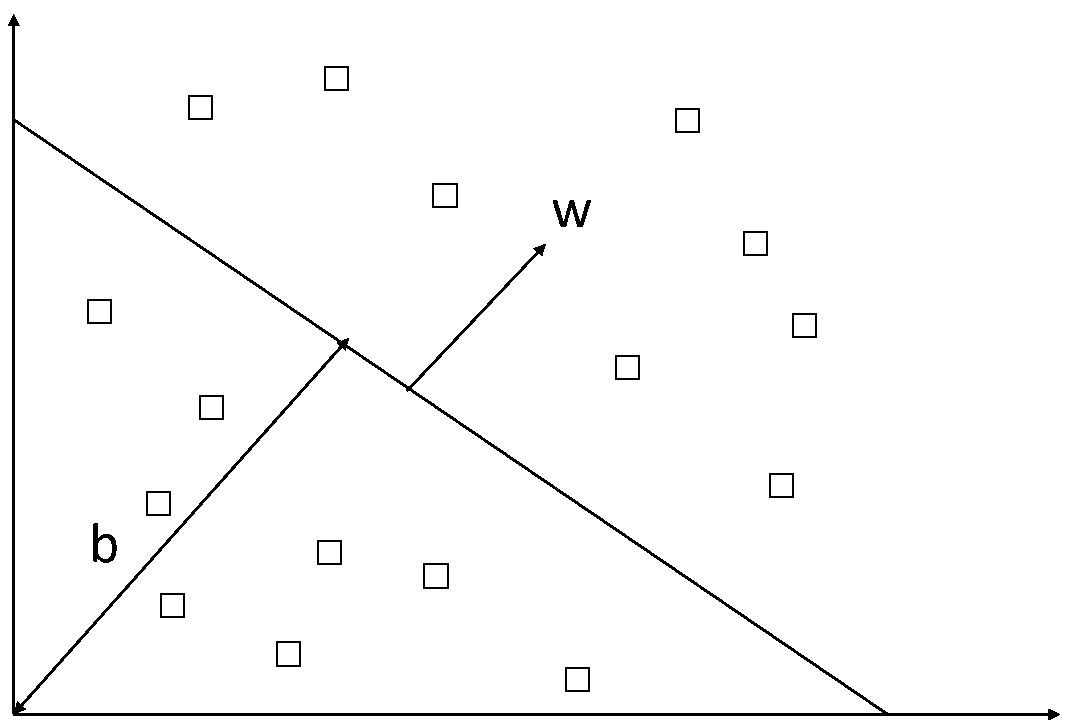
\includegraphics[clip,width=7.0cm]{./images/heimen.png}
    \caption{2次元サンプルにおける入力特徴と識別平面}
    \label{fig:heimen}
  \end{center}
\end{figure}


\section{マージン最大化}
線形しきい素子を用いて,線形分離が可能な訓練サンプル集合Sについて考える.この訓練サンプル集合Sは,
線形しきい素子のパラメータをうまく調節することにより,訓練サンプル集合を誤りなく分けることが可能である.
しかし,訓練サンプル集合が線形分離可能であるとしても,一般には,訓練サンプル集合を誤りなく分けるパラメータを一意に定めるのは難しい.

SVMでは,このパラメータを求める手法としてマージン最大化と呼ばれる方法を使用する.マージン最大化とは,
最も近い訓練サンプルとの距離をマージンと定義し,マージンが最大になるような識別平面を求める手法である.
訓練サンプルをすれすれに通るのではなく,なるべく余裕を持って分離することが可能な識別平面を求めることができる.
この2次元訓練サンプル集合におけるマージンを図\ref{fig:margin}に示す.

\begin{figure}[htbp]
  \begin{center}
    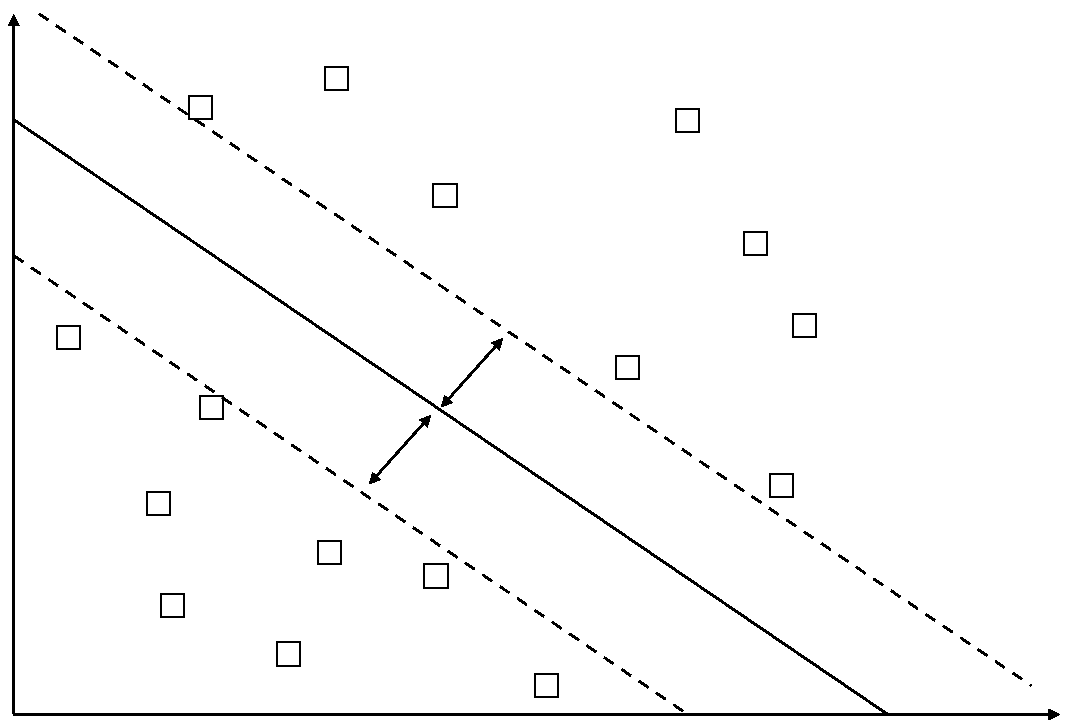
\includegraphics[clip,width=7.0cm]{./images/margin.png}
    \caption{2次元サンプルにおけるマージン}
    \label{fig:margin}
  \end{center}
\end{figure}

N個の特徴ベクトル $ x_1,x_2, ... ,x_{N-1},x_N $ と,それぞれのサンプルに対する正解のクラスラベル $ t_1,t_2, ... ,t_{N-1},t_N $
を持った,訓練サンプル集合Sにおいて,Sが線形分離可能な場合には,以下の式(4.3)を満たすパラメータが存在する.

\begin{equation}
     t_i (w_i x_i + b) \geq 1 (i = 1,2,...,N-1,N)
\end{equation}

これは、図\ref{fig:margin}上の2つの点線 $ ((w \cdot x) + b = \pm 1) $ で定義される2つの超平面より、全ての訓練サンプルが完全に分離しており,2つの超平面の内側にはサンプルが1つも存在しないことを意味している.このとき,識別平面とこの2つの超平面との距離(マージンの大きさ)は,$ \frac{1}{||w||} $ と表現される.

\newpage

つまり,マージン最大化を満たすパラメータ , を求める問題は,以下の式(4.4)に示す,目的関数$ L(w) $を最小化する問題として考えることができる.

\begin{equation}
     L(w) = \frac{1}{2} ||w||^2
\end{equation}

この目的関数の最適化問題は,数理計画法の分野において2次計画問題に帰着することができる.そのため最適解が1つに定まるようになる.その結果,分類問題における問題の1つである局所的最適解に陥ることがなくなることがわかる.

\section{サポートベクタ}
SVMでは,訓練の際に分離平面を構成する特徴ベクトルを選び出し,サポートベクタとする.これにより,計算量の削減を行うことができる.これは訓練が完了した段階に,識別平面を構成するために必要なマージンの小さい特徴ベクトルを最小限の数だけ確保することにより実現する.この特徴ベクトルをサポートベクタと呼ぶ.分類の段階において,識別平面を構成するときには,このサポートベクタとそれに伴うパラメータのみを使用する.図\ref{fig:sapo}では,2つの超平面に接している点Aがサポートベクタである.

\begin{figure}[htbp]
  \begin{center}
    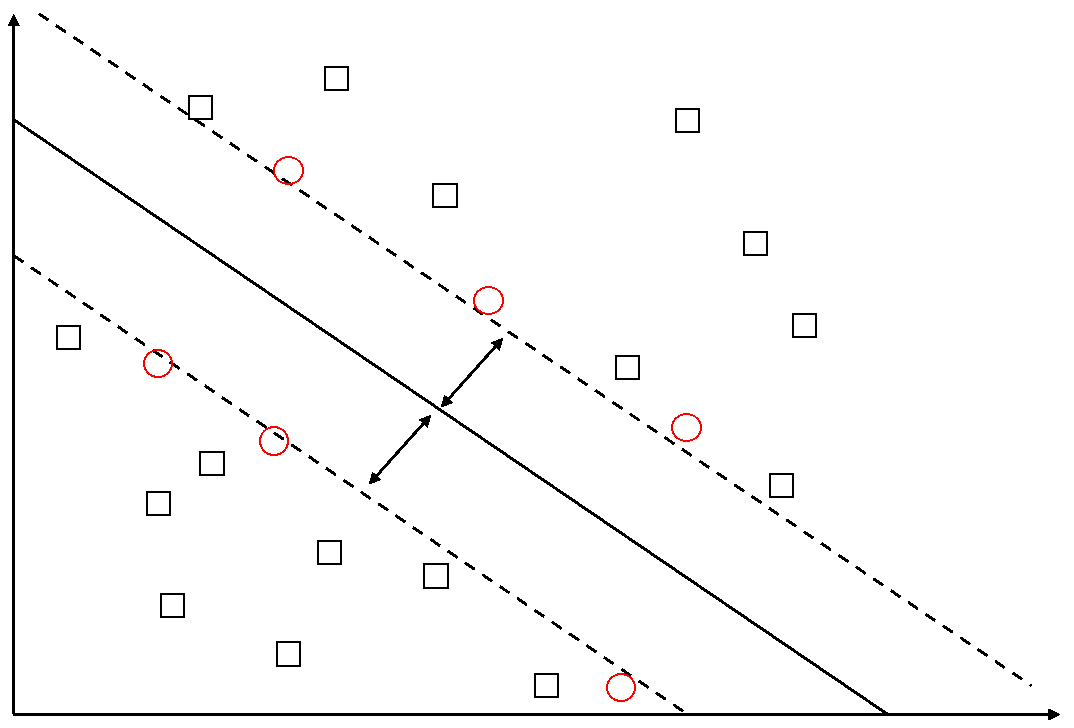
\includegraphics[clip,width=7.0cm]{./images/sapo.png}
    \caption{サポートベクタの例}
    \label{fig:sapo}
  \end{center}
\end{figure}

\newpage

\section{ソフトマージン}
前節までは,線形分離が可能な訓練サンプル集合を例に挙げてSVMの概要,識別,学習方法について述べた.しかしながら,パターン認識の実問題で線形分離可能な場合は少ない.故に,実際的な問題にSVMを使用するには,工夫が必要である.そこで,完全な線形分離ができなくても,多少の識別誤りを許容するように制約を緩め,最適な識別平面を求める方法である,ソフトマージンについて説明する.

マージン最大化では,式(4.3)を制約条件としている.この場合には,2つの超平面によってデータを完全に分離することが可能なため,2つの超平面の間にデータは存在しない.ソフトマージンでは,いくつかのデータが超平面を超えて,超平面の内側に入ることを許容する.図\ref{fig:softma}で示されるように,識別平面を超えた位置にデータが存在する場合を想定している.これにより,ノイズや誤りによって線形分離が不可能な入力データに対しても識別平面を構成することが可能になる.

\begin{figure}[htbp]
  \begin{center}
    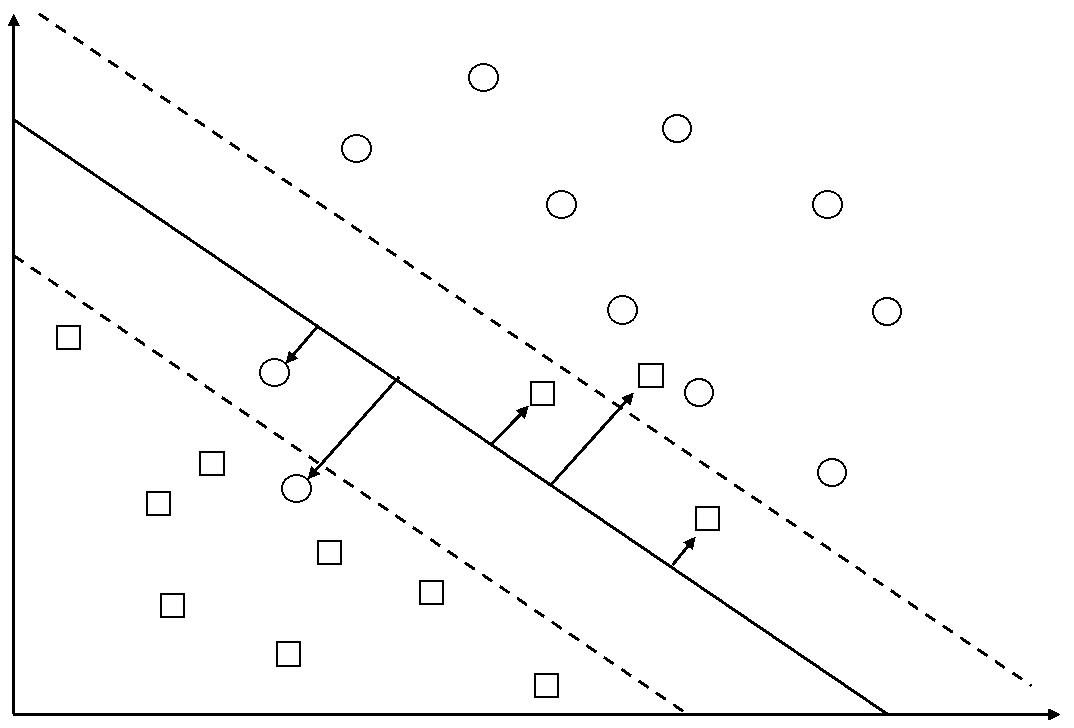
\includegraphics[clip,width=7.0cm]{./images/softma.png}
    \caption{ソフトマージンの例}
    \label{fig:softma}
  \end{center}
\end{figure}

\newpage

ノイズや誤りによって,誤った領域に存在している訓練サンプルの識別平面からの距離を,誤り量のパラメータ$ ε_i (\geq 0) $を用いて,$ \frac{ε_i}{||w||}$と表すと,誤ったサンプルの総和は式(4.5)のようになる.

\begin{equation}
      \sum_{i=1}^N \frac{ε_i}{||w||}
\end{equation}

となる.式(4.5)は誤り量なので,なるべく小さい値となることが望ましい.このとき,誤り量のパラメータ$ ε_i $を用いて,最適な識別面を求める制約条件は式(4.6)となる.

\begin{equation}
      ε_i (\geq 0), t_i(w_i x_i + b) \geq 1 - ε_i (i = 1,2,...,N-1,N)
\end{equation}

この条件の下で,式(4.7)で示す目的関数$ L(w,ε) $を最小化すればよい.

\begin{equation}
      L(w,ε) = \frac{1}{2} ||w||^2 + γ\sum_{i=1}^Nε_i
\end{equation}

この目的関数では,パラメータγを用いて,第1項のマージンの大きさと,第2項の誤り距離の優先比率の調整を行う.

\newpage

\section{カーネルトリック}
前節のソフトマージンを用いることで,線形分離可能でない場合に対して,線形しきい素子のパラメータを求めることが可能である.しかし,本質的に非線形で複雑な識別問題への適用は不可能である.非線形問題に対応するための方法として,カーネルトリック[4]を使用する.特徴ベクトルを非線形変換して線形識別をしやすい高次元特徴空間に写像し,線形識別を行う.写像した先で線形識別を行うことは,もとの空間で識別関数を構成することに対応する.図\ref{fig:kouji}は特徴ベクトルxを写像$ \phi(x) $によって変換し,線形分離しやすくした例である.

\begin{figure}[htbp]
  \begin{center}
    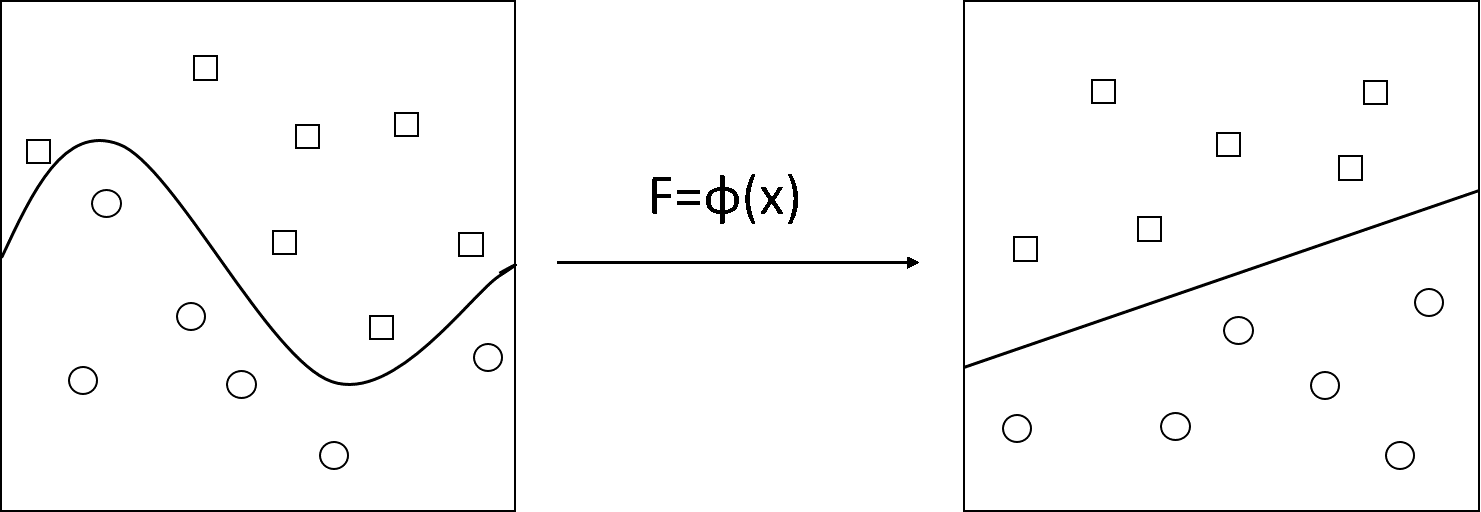
\includegraphics[clip,width=7.0cm]{./images/kouji.png}
    \caption{高次元特徴空間への変換の例}
    \label{fig:kouji}
  \end{center}
\end{figure}

しかし,高次元への写像を行うと次元の増加に伴い汎化能力が落ちてしまう.また,難しい問題を線形分離可能にするためには,訓練サンプルと同程度の大きな次元に写像しなければならない.そのため,膨大な計算量が必要になる.そこでカーネルトリックの利用を考える.

SVMでは,識別関数が入力パターンの内積のみに依存しており,内積を計算すれば最適な識別関数を構成することが可能である.高次元空間での2つの要素$ \phi(x_1)$と$ \phi(x_2)$の内積を式(4.8)と定義する.

\begin{equation}
      \phi(x_1) \cdot \phi(x_2) = K(x_1,x_2)
\end{equation}

非線形写像によって変換された高次元空間での特徴$ \phi(x_1)$や$ \phi(x_2)$の計算する変わりに,$K(x_1,x_2)$から最適な非線形写像を構成できる.このような$ K $のことをカーネルと呼ぶ.このように高次元に写像しながら,実際には写像された高次元空間上での特徴の計算を避け,カーネルの計算のみで最適な識別関数を構成する.この一連の操作がカーネルトリックである.実用的には, は計算が容易なものが望ましい.

\newpage

カーネルトリックを利用して,高次元空間に射影したときの線形分離の制約条件は,式(4.9),式(4.10)に示す.

\begin{equation}
      t_i(\phi(w_i) \cdot \phi(x_i) + b) \geq 1, (i = 1,2,...,N-1,N)
\end{equation}

\begin{equation}
      t_i(K(w_i,x_i) + b) \geq 1, (i = 1,2,...,N-1,N)
\end{equation}


写像空間はカーネル$K$の種類によって異なるため,分離しやすい高次元空間上に射影が行われるようにカーネル$K$を選択しなければならない.こここでは,代表的なカーネルを3つ以下に示す.

●多項式カーネル

定数$c>0$,次数を$d$とする多項式カーネルを式(4.11)に示す.

\begin{equation}
      K(x_i,x_j) = (x_i \cdot x_j + c)^d
\end{equation}

●ガウシアンカーネル

データに関する事前知識がない場合に用いられる汎用的なカーネルである.$σ^2(σ>0)$は分散を示す.

\begin{equation}
      K(x_i,x_j) = \exp(-\frac{||x_i - x_j||^2}{2σ^2})
\end{equation}

\begin{figure}[htbp]
  \begin{center}
    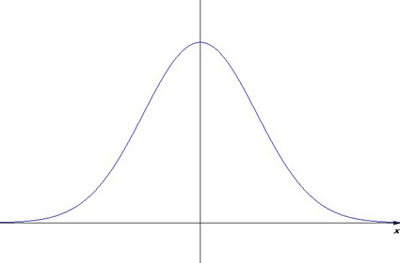
\includegraphics[clip,width=7.0cm]{./images/gaus.png}
    \caption{ガウス関数}
    \label{fig:gaus}
  \end{center}
\end{figure}

\newpage

●シグモイドカーネル
主に,ニューラルネットワークの代わりに使用されるシグモイドカーネルを用いることにより,SVMとニューラルネットワークが表層的に類似したものになるためである.

\begin{equation}
      K(x_i,x_j) = \tanh(cx_i \cdot x_j + θ)
\end{equation}

\begin{figure}[htbp]
  \begin{center}
    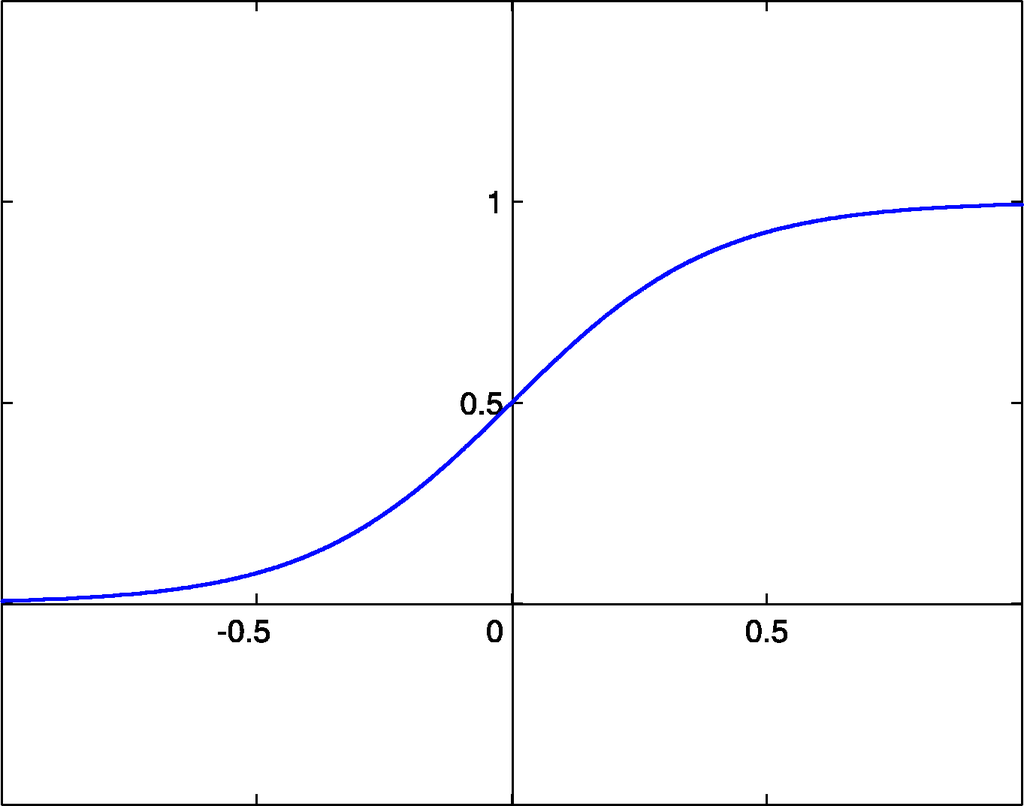
\includegraphics[clip,width=7.0cm]{./images/sigu.png}
    \caption{シグモイド関数}
    \label{fig:sigu}
  \end{center}
\end{figure}


